\section{Using a Virtual Machine}

Just like a tree-walking interpreter, a virtual machine presents a way of implementing an interpreter for a programming language.
However, the way a virtual machine operates fundamentally differs from a tree-walking interpreter.
For rush, we have implemented a virtual machine backend in order to compare it to the previously explained tree-walking interpreter.

\subsection{Defining a Virtual Machine}

Often, one might encounter the term \emph{virtual machine} when talking about emulating an existing type of computer using a software system.
This emulation often includes simulating additional devices like the computer's display or its disk.
In this context however, a \emph{virtual machine}\footnote{May later be shortened to \enquote{VM}} is a software entity which emulates how a computer interprets instructions.
Just like a real computer, a virtual machine executes low-level instructions directly.
Therefore, the VM is unable to traverse the AST and therefore relies on a compiler to generate its input instructions.

Since a physical processor and a virtual machine share some fundamental traits,
the architecture of a virtual machine is often a slight deviation from the \emph{von Neumann architecture}.
The von Neumann architecture was first introduced by John Neumann in the year 1945.
Von Neumann originally presented a design which allows implementing a computer using relatively few components.
Following the von Neumann architecture, a processor would usually contain components like an \emph{ALU}\footnote{Short for \enquote{arithmetic logic unit}}, a control unit, multiple registers, memory, and basic IO~\cite[p.~172]{Ledin2020-yp}.
The ALU is often designed so that it performs logical and mathematical operations as fast as possible.
However, to keep its implementation simple, it lacks the ability to fetch and execute instructions from memory directly.
Therefore, the processor contains a control unit which manages the \emph{fetch-decode-execute} cycle.
The fetch-decode-execute cycle is a simplification of the steps a processor performs in order to execute an instruction.
The list below explains the individual steps of the fetch-decode-execute cycle.

\begin{itemize}
	\item \textbf(Fetch): The processor's control unit loads the next instruction from the adequate memory location.
	      The instruction is then placed into the processor's internal instruction register where it is available for further analysis.
	\item \textbf(Decode):
	      The processor's control unit examines the fetched instruction in order to determine if additional steps must be taken before or after instruction execution.
	      Such steps may involve accessing additional registers or memory locations.
	\item \textbf(Execute):
	      The control unit dispatches the instruction to a specialized component of the processor.
	      The target component is often dependent on the type of instruction since each processor component is optimized with one specific type of instruction in mind.
	      For instance, the control unit may invoke the ALU in order to execute a mathematical instruction.
\end{itemize}

A computer's processor performs this fetch-decode-execute cycle repeatedly from the moment it is powered on until the point in time when it is powered down again.
For relatively simple processors, each cycle is executed in an isolated manner because instructions are executed in a sequential order.
This means that the execution of the instruction $i$ is delayed until execution of $i - 1$ has completed~\cite[pp.~208-209]{Ledin2020-yp}.

For virtual machines, executing the input instructions in sequential order is often also the simplest solution.
Often, a virtual machine executes instructions similarly to the fetch-decode-execute cycle.
Although the von Neumann architecture is relatively simple, one does not always have to adopt it when implementing a virtual machine.
Since virtual machines are purely abstract constructs, meaning that they are implemented using software, design constrains are usually kept to a minimum.
Therefore, a virtual machine can also be implemented with the high-level constructs of the source language in mind.
For instance, the VM might feature specialize break, continue, or loop instructions which are not present in modern-day CPUs.
Designing the architecture of a virtual machine can sometimes be a challenging task since choosing an adequate set of features may involve a lot of testing iterations.
Because neither the compiler nor the VM exist in the beginning, one should carefully plan the implementation of their VM's architecture.
From the point where the architecture is clear, implementation of the VM should normally be a straight-forward task.

\subsection{Register-Based and Stack-Based Machines}

One of the main decisions to be made when designing a VM is how it implements temporary storage.
Physical processors often use \emph{registers} in order to make larger computations feasible.
Registers are a limited set of very fast, low capacity storage units.
On modern architectures, like \emph{x86\_64}, each general-purpose register is able to hold as much as 64 bits of information.
However, there is always only a limited amount of registers available since they are physical components of the computers CPU\@.
Therefore, programs often only utilize registers for storing temporary values, such as intermediate results of a large computation.
The main alternative to using registers is a stack-based design.
A popular example for a stack-based virtual machine is \emph{WebAssembly}~\cite[p.~44]{Sendil2022-fy}.
For more information on WebAssembly, we will present a compiler targeting WebAssembly in Chapter~\ref{chap:high_level_targets}.
For compiler writers, register allocation is often a demanding task.
This problem is described in more detail in Chapter~\ref{chap:low_level_targets}.
Since register allocation is not required in a compiler targeting stack-based machines, its implementation is often significantly easier compared to a compiler targeting a register-based machine.
Therefore, one might choose to implement a stack-based virtual machine in order to minimize complexity of both the compiler and the interpreter.
However, a stack-based design also introduces several issues on its own.
For example, register-based machines might regularly outperform stack-based machines.
A reason for this is that use of the stack usually requires a lot of push or pop operations which could have otherwise been omitted.

\subsection{Comparing the VM to the Tree-Walking Interpreter}
One significant benefit of virtual machines is that they execute programs much faster compared to most tree-walking interpreters.
A reason for this speedup is that tree-traversal involves a lot of overhead which is omitted when instructions are interpreted directly.

The code in Listing~\ref{lst:rush_vm_faster} displays a recursive function implemented in rush.

\TSListing[ranges={5-11}, caption={A Recursive rush Program}, label={lst:rush_vm_faster}, float=H]{listings/vm_faster.rush}

\noindent
\begin{figure}[h]
	\begin{minipage}{.7\textwidth}
		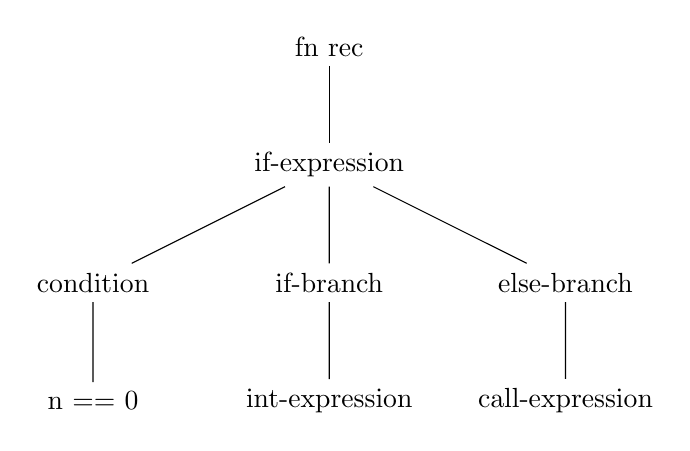
\begin{tikzpicture}[
				tlabel/.style={pos=0.4,right=-1pt,font=\footnotesize\color{red!70!black}},
			]
			\node{fn rec}
			child { node {if-expression}
					child { node {condition} child {node {n == 0}} }
					child [missing]
					child { node {if-branch} child {node {int-expression}} }
					child [missing]
					child { node {else-branch} child{node{call-expression}} }
				};
		\end{tikzpicture}
	\end{minipage}%
	\begin{minipage}{.3\textwidth}
        \TSListing[raw=true, fancyvrb={frame=none}]{listings/vm_faster_instructions.txt}
	\end{minipage}
	\caption{Abstract Syntax Tree and VM Instructions of a Recursive rush Program}\label{fig:tree_vs_vm}
\end{figure}

Figure~\ref{fig:tree_vs_vm} displays a heavily simplified syntax tree and rush VM instructions representing the function displayed in Listing~\ref{lst:rush_vm_faster}.
The root node of the tree represents the \texttt{rec} function.
Since the function only contains a single expression, the if-expression node is the only child of the root node.
The if-expression contains a condition, an if-branch, and an else-branch.
Since the function should not call itself again if \texttt{n} is equal to 0, the if-branch returns 0.
In the else-branch however, the \texttt{rec} function calls itself recursively.
When the above program is executed using the tree-walking interpreter, the algorithm traverses the entire tree of the \texttt{rec} function every time it recurses.
Since \texttt{rec} is a recursive function, the tree-walking interpreter would have to traverse it $n$ times.
In this example, the AST of the program is relatively simple.
However, the complexity of the tree grows as the source program evolves.
Since loops and recursive functions execute the code in their bodies repeatedly, the tree traversal of the body presents an inefficiency.
Here, the inefficiency solely lies in the repeated tree-traversal, not in the repetition introduced by an iterative or recursive algorithm.
In order to improve efficiency, an algorithm could traverse the AST once, saving its semantic meaning in the process.
Then, the semantic meaning of the previously traversed tree could be interpreted repeatedly without the additional overhead.
This behavior is used in the rush VM since it interprets instructions previously generated by a compiler.
A compiler targeting the virtual machine's architecture first traverses the AST and outputs a sequence of instructions.
The instructions on the right side of Figure~\ref{fig:tree_vs_vm} represent the program in Listing~\ref{lst:rush_vm_faster}.
Every time the \texttt{call} instruction in line 23 is executed, the VM only needs to jump to the instruction in line 10 in order to execute the \texttt{rec} function recursively.
Since repeated traversal of the syntax tree is omitted, rush programs will run significantly faster using the VM compared to the tree-walking interpreter.
Using the VM, executing the \texttt{rec} function using an input of $n = 1000$ took around 160 $\mu$s.
However, executing the identical code using the tree-walking interpreter took around 427 $\mu$s\footnote{Average from 10000 iterations. OS: Arch Linux, CPU: Ryzen 5 1500, RAM: 16 GB}.
Therefore, the rush VM executed the identical code roughly 2.6 times faster than the tree-walking interpreter.
However, the initial delay caused by compilation is not considered in this benchmark.

\subsection{The rush Virtual Machine}

The rush virtual machine is a stack-based interpreter implemented using the Rust programming language.
The machine's architecture is completely fictional and includes a \emph{stack} for storing short-term data, \emph{linear memory} for storing variables, and a \emph{call stack} for managing function calls.
Like most virtual machines, the rush VM uses a fetch-decode-execute cycle in order to interpret its programs.

\TSListing[ranges={16-26}, caption={Struct Definition of the Vm}, label={lst:vm_struct}, float=H]{deps/rush/crates/rush-interpreter-vm/src/vm.rs}

Listing~\ref{lst:vm_struct} displays the struct definition of the rush VM\@.
In line 18, a field called \texttt{stack} is defined.
Like explained above, the rush VM uses a stack for storing temporary values.
Even though the stack is implemented using a \texttt{Vec}, it behaves identical to a LIFO stack data structure.
In line 20, the \texttt{mem} field is declared.
This field represents the linear memory capable of storing variables.
However, each memory cell is implemented to hold an option of a value.
Therefore, each memory cell may also hold a \texttt{None} value representing uninitialized memory.
In line 23, the \texttt{mem\_ptr} field is declared.
It, too, serves an important role in managing the linear memory.
The exact responsibilities of the so-called \emph{memory pointer} will be explained shortly.
Lastly, the \texttt{call\_stack} is declared.
This field also behaves like a stack and is responsible for managing function calls and returns.
The instructions in Figure~\ref{fig:tree_vs_vm} can be interpreted by the rush VM\@.
Here, the output program is structured as functions which each contain a list of their instructions.
Since function and variable names are replaced by indices, strings can be entirely omitted in the output instructions.
This often leads to a decrease in code size and an increase in runtime speed.
For better understanding, we have annotated the individual functions with their human-readable names.

The first block of instructions can be called the \emph{prelude} since its only task is to call the \texttt{main} function and declare global variables.
Global variables need to be initialized at the beginning of a program so that they can be accessed later in the program.
If global variables were present in the example, the prelude would contain the instructions used for initializing them.
If the prelude was omitted, the main function would instead contain these instructions since it is executed at program start.
However, recursion of the \texttt{main} function is legal in rush.
Therefore, each time the \texttt{main} function recurses, all global variables would be restored to their initial values.
In order to prevent this bug, the rush VM uses a prelude function which is guaranteed to run only once.

Linear memory in the VM is represented as an array which saves the runtime value of a variable in each index.
Since an array is used, the memory of the VM is limited.
However, a large memory size if often enough to run most of the possible programs.
In the rush VM, each storage cell can be accessed using two addressing modes.
When using the \emph{absolute addressing} mode, the exact index of the memory cell is specified.
For instance, if the value of variable \texttt{d} of Figure~\ref{fig:rush_vm_linmem} was to be retrieved, the VM would need to access the storage cell with the index 4.
However, the absolute position of a variable in memory can only be determined at runtime.
In a recursive function, each recursion adds more variables to the scope, thus allocating more memory.
Here, the exact number of recursions the function performs would have to be known at compile time.
Of course, this presents an impossible task, thus making writing a compiler targeting the VM impossible.
However, the rush VM also implements a \emph{relative addressing} mode which can be used without knowledge about the absolute position of the memory cell.
For instance, the variable \texttt{d} can be addressed by index 0 using the relative addressing mode.
In Figure~\ref{fig:rush_vm_linmem}, the memory pointer (shortened to \enquote{mp}) is set to 4.
Considering the value of the memory pointer, the absolute address of any relative address can be calculated at runtime.
Here, the absolute address $a$ is the sum of the relative index $i$ and the runtime memory pointer $m$.
Therefore, the absolute address of any relative address can be calculated at runtime like this: $a = i + m$.
By also implementing this relative addressing mode,
compilers targeting the rush VM can generate code without knowing the runtime behavior of a program.

\begin{figure}[h]
	\includegraphics[width=\textwidth]{./vm_linmem_draft.png}
	\caption{\textcolor{red}{DRAFT:} Linear Memory of the rush VM}\label{fig:rush_vm_linmem}
\end{figure}

In order to get a deeper understanding of the addressing modes, a practical example can be considered.
The code in Listing~\ref{lst:rush_pointer_simple} displays a rush program in which a pointer to a variable is created.
First, the integer variable \texttt{num} is created.
In line 3, a pointer variable called \texttt{to\_num} is created by \emph{referencing} the \texttt{num} variable.

\TSListing[caption={Minimal Pointer Example in rush}, label={lst:rush_pointer_simple}, float=H]{listings/simple_pointer.rush}

In the rush VM, absolute addressing is only used for global variables and pointers.
Since a pointer specifies the address of another variable, its runtime value will be the absolute address of its target variable.
In the VM, the absolute address of a variable is calculated as soon as it is referenced using the \texttt{\&} operator.
For this purpose, the \texttt{reltoaddr} instruction exists.
This instruction calculates the absolute address of its operand and pushes the result onto the stack.
Here, the operand is the relative address of the variable to be referenced.
Listing~\ref{lst:rush_pointer_simple_vm_instructions} shows the VM instructions generated from the rush program in Listing~\ref{lst:rush_pointer_simple}.

\TSListing[raw=true, caption={VM Instructions for the minimal Pointer Example}, label={lst:rush_pointer_simple_vm_instructions}, float=H]{listings/vm_instructions_simple_pointer.txt}

The first instruction \texttt{setmp} (\emph{set memory pointer}) increases the memory pointer by two.
This is because the \texttt{main} function contains two local variables whose space is to be allocated at the start of the function.
For instance, one might encounter \texttt{mp} being incremented by 0 since the corresponding function contains no local variables.
The next instruction \texttt{push} pushes the value 42 onto the stack.
In line 4, the \texttt{svari} (\emph{set variable immediate}) assigns the top value on stack to the specified relative address.
Here, 42 is popped off the stack since it is used by the \texttt{svari} instruction.
Next, the instruction stores the previously popped value at the relative address at the relative address 0 specified in the operand.
Now, the variable \texttt{num} with an initial value of 42 has been created.
Next, the \texttt{to\_num} variable is created by referencing the \texttt{num} variable.
In line 5, the \texttt{reltoaddr} (\emph{relative to address}) instruction is used to calculate the absolute memory address of the \texttt{num} variable.
This instruction calculates the absolute address of its operand at runtime using the algorithm described above.
Then, the instruction pushes the calculated address onto the stack so that it can be used by following instructions.
Here, the relative address 0 is used since the \texttt{svari} instruction has previously saved 42 at this location.
Therefore, the value of the variable \texttt{num} is saved at the relative address 0.
In line 6, the \texttt{svari} instruction is used again.
This time, it is used to save the value of the \texttt{to\_num} variable.
Since the absolute address of the referenced variable was previously calculated, it now exists on top of the stack.
Now, the instruction saves the absolute address of \texttt{num} at the relative address -1.
This is because the compiler targeting the VM assigns variables to higher relative addresses first.
The compiler then progresses into lower relative memory as more variables of the function are declared.
To summarize the above paragraph, this example uses relative addressing in order to declare local variables of a function.
However, absolute addressing is also used when variables are referenced in order to create pointers.
Therefore, each addressing mode serves a separate and important purpose.

\subsection{How the Virtual Machine Executes A rush Program}

By considering the minimal pointer example from above, we now have a rough idea how the VM might execute instructions.
In order to get a better understanding of how the rush VM works exactly, we will explain how it executes the program in Listing~\ref{lst:rush_vm_faster}.
For this, we should consider the instructions in Figure~\ref{fig:tree_vs_vm} again.
The first instruction of the prelude function is \texttt{setmp}.
This instruction adjusts the memory pointer by the amount specified in the instruction's operand.
In this case however, the memory pointer remains unmodified since the operand of the instruction is 0.
Next, the \texttt{call 1} instruction calls the \texttt{main} function.
In order to understand how function calls work in this VM, we must consider the call stack of the rush VM\@.
Before the call-instruction, the caller pushes any call-arguments onto the stack so that they can be used as parameters by the callee.
Figure~\ref{fig:rush_vm_call_stack} displays the state of the VMs call stack after the \texttt{call 1} instruction has been executed.
During execution of a call-instruction, the VM pushes a new stack frame onto its call stack.
Listing~\ref{lst:call_frame_struct} shows how a call frame is implemented.

\TSListing[ranges={26-31}, caption={Struct Definition of a \texttt{CallFrame}}, label={lst:call_frame_struct}, float=H]{deps/rush/crates/rush-interpreter-vm/src/vm.rs}

In this implementation, each call frame holds two important pieces of information.
In line 28 of Listing~\ref{lst:call_frame_struct}, the \texttt{ip} field is declared.
It specifies the \emph{instruction pointer} which holds the index of the current instruction.
Since the \texttt{call} instruction was interpreted previously, the instruction pointer of the new call frame is set to 0 as execution should continue at the first instruction of the called function.
The \texttt{fp} field is declared in line 30.
This field specifies the \emph{function pointer} which holds the index of the current function.

After the function call, \texttt{fp} is set to 1 since the main function is called and instruction should start at the first instruction of the main function.
Figure~\ref{fig:rush_vm_call_stack} shows how the call stack of the VM looks like after the \texttt{call} instruction has been interpreted.
Function calls are managed in a stack in order to allow returning from functions.
If the VM encounters a \texttt{ret}\footnote{Short for \enquote{return}} instruction, it should leave the current function.
However, it should also know where to resume its fetch-decode-execute cycle.
For this, the VM just simply pops the top element from its call-stack.
Now, the top element on the stack contains the call-frame of the caller function.
In this call frame, \texttt{ip} still points to the \texttt{call} instruction which was responsible for calling the function.
Since \texttt{ip} is incremented automatically after most instructions, the VM resumes instruction execution at the first instruction after the call-instruction.
This way, function calls are implemented in a simple but robust manner.

\begin{figure}
	\centering
	\begin{tikzpicture}
		\node[stack=3, rectangle split part align=center, text width=10ex, text centered, inner xsep=0]{
			\shortstack{prelude\\$fp=0$\\$ip=1$}
			\nodepart{two}{\shortstack{main\\$fp=1$\\$ip=0$}}
			\nodepart{three}{\ldots}
		};
	\end{tikzpicture}
	\caption{Call Stack of the rush VM}\label{fig:rush_vm_call_stack}
\end{figure}

Now that the call-instruction has been interpreted, the VM begins executing the first instruction of the main-function.
Since the main-function only calls the \texttt{rec} function with the argument 1000, there are no new concepts to consider in this function.
After the call instruction in line 7, the VM starts executing the instructions of the \texttt{rec} function.
At the beginning of the \texttt{rec} function, the memory pointer is incremented by 1.
This might seem erroneous since the \texttt{rec} function contains no visible variable declarations in its body.
However, this behavior is correct since function parameters count as variable declarations.
Since the function takes one parameter, the memory pointer is incremented by one cell.
Next, the instruction \texttt{svari} saves the value of the parameter which was previously pushed onto the stack at the relative address 0.
In line 12, the relative address of the memory cell containing the value of the parameter is pushed onto the stack.
It is then consumed by the \texttt{gvar} instruction in line 13.
At this point the top element on the stack contains an address-value referring to the target of the \texttt{gvar} instruction.
Therefore, the instruction first pops the top element from the stack.
In this case, the value of the popped element is the relative address 0.
Then, the instruction retrieves the value of the target variable and pushes it onto the stack.

In line 14, the constant value 0 is pushed onto the stack.
Next, the \texttt{eq} instruction pops two elements from the stack in order to test them for equality.
Then, the result of the comparison is pushed onto the stack as a boolean value.
In this case, the instruction compares if the current value of \texttt{n} is equal to 0.
In line 16, the \texttt{jmpfalse} instruction is executed.
This instruction jumps to the specified instruction index if the value on top of the stack is \texttt{false}.
In this case, if the value on the stack is false, the parameter \texttt{n} was not equal to 0.
Now, the VM would jump to the instruction in line 19.
Here, the value of the parameter \texttt{n} is pushed onto the stack using the previously explained \texttt{push} and \texttt{gvar} instructions.
Now, the top item on the stack is the value of the parameter \texttt{n}.
In line 21, the \texttt{push} instruction pushes a constant 1 onto the stack.
Next, the \texttt{sub} instruction pops the first two elements from the stack in order to subtract their values from each other.
In this case, the instruction subtracts 1 from the value of \texttt{n} and pushes the result onto the stack.
Next, the \texttt{rec} calls itself recursively using a previously explained \texttt{call} instruction.
Since the call argument is the top element on the stack, the result of the subtraction is used as the argument of the recursive call.
Next, the function decrements the memory pointer in order to deallocate used memory using the \texttt{setmp} instruction in line 24.
At the end of a function, the memory pointer is always decremented by the amount it was incremented at the beginning of the function.
By deallocating the now unused memory, the compiler prevents the code from leaking memory at runtime.
Lastly, the \texttt{ret} instruction is used to return from the function.
Now we have considered what happens if the value of \texttt{n} was not equal to 0.

However, if the result of the comparison in line 15 is true, meaning that \texttt{n} is equal to 0, the \texttt{jmpfalse} instruction in line 16 does nothing.
In this case, the VM continues to the \texttt{push} instruction in line 17.
Here, the constant value 0 is pushed onto the stack.
Next, the VM interprets the \texttt{jmp} instruction in line 18.
Unlike \texttt{jmpfalse}, this instruction performs its jump without any condition.
In this case, the instruction jumps to the instruction at index 14 of the current function.
The instruction at index 14 is \texttt{setmp} in line 24.
Since functions also return values by placing them on top of the stack, the return-value would be 0 in this case.
Since we have covered what the instructions in the lines 24 and 25 do, we can summarize that the function returns the value 0 in this case.

Now that we have explained the semantic meaning of the instructions in Figure~\ref{fig:tree_vs_vm}, we will explain how the fetch-decode-execute cycle works in the VM\@.
The code in Listing~\ref{lst:vm_run_meth} displays the \texttt{run} method of the rush VM\@.

\TSListing[ranges={168-179}, caption={The \texttt{run} Method of the rush VM}, label={lst:vm_run_meth}, float=H]{deps/rush/crates/rush-interpreter-vm/src/vm.rs}

This method manages the entire fetch-decode-execute cycle of the VM\@.
It is immediately apparent that this method looks relatively simple considering that it plays such of a fundamental role in the VM\@.
Since the fetch-decode-execute cycle executes instructions repeatedly, the main construct in the function is a while-loop.
The condition of the loop checks that the current instruction pointer refers to a legal instruction inside the current function.
This way, the VM comes to a halt if it reaches the end of an instruction sequence.
In line 168, the next instruction to be interpreted is saved as the variable \texttt{instruction}.
This line represents the \emph{fetch} step since the next instruction is fetched from memory and placed in a spot where it can be used by the following steps.

In the body of the loop, the current instruction is executed using the \texttt{self.run\_instruction} method.
This method can return a runtime error, such as an integer-overflow error.
Furthermore, this method may return an integer representing the exit code of the program.
However, if the method returns none of these two possible types, the fetch-decode-execute cycle continues.
In this code however, one cannot observe the instruction pointer being incremented.
In order to answer the final question of how the current instruction is executed, and the instruction pointer is incremented, we will now examine the code in Listing~\ref{lst:vm_run_instr_meth}.

\TSListing[ranges={347-359}, caption={Parts of the \texttt{run\_instruction} Method of the rush VM}, label={lst:vm_run_instr_meth}, float=H]{deps/rush/crates/rush-interpreter-vm/src/vm.rs}

The code in Listing~\ref{lst:vm_run_instr_meth} displays the last part of the \texttt{run\_instruction} method.
This method mainly consists of an algorithm mathing the current instruction in order to execute specific code representing the instruction's semantic meaning.
In this example, the implementations of the \texttt{bitand} and \texttt{bitxor} instructions are visible.
Both instructions first pop two elements from the stack since they represent the operands of the underlying logical computation.
Then, a corresponding helper function is invoked on the left hand side operand.
The helper function then performs the actual computation of the logical operation.
Most of the infix-expressions are later executed similarly.
It is apparent that the execution of these instructions involves relatively little difficulty.
After the instruction has been executed, the instruction pointer is finally incremented and nothing is returned.
For some special instructions, such as the jump-instructions, the instruction pointer should not be incremented since it would interfere with the jump.

\TSListing[ranges={191-194}, caption={Execution of the \texttt{jmp} Instruction in the rush VM}, label={lst:vm_jmp_instr}, float=H]{deps/rush/crates/rush-interpreter-vm/src/vm.rs}

As seen in Listing~\ref{lst:vm_jmp_instr}, the \texttt{jmp} instruction only sets the instruction pointer to the target index specified in the instruction operand.
Then, the code returns from the method so that the instruction pointer is not incremented later.
This method represents both the \emph{decode} and \emph{execute} step since it first matches (\emph{decode}) and then interprets (\emph{execute}) the current instruction.
Now that we have explained how some important parts of the rush VM work,
the question of how its input instructions are generated remains.
Therefore, the compiler targeting the rush VM is presented in the next chapter.

As a conclusion, a VM is often a reasonable approach if an interpreted programming language is to be implemented.
The main advantages of a VM are increased speed and reduced memory usage at runtime.
The downsides include the need for a compiler targeting the VM, thus making its implementation more demanding compared to a tree-walking interpreter.
